\chapter{Science of ice reservoirs}
\label{chap:science}

\cleanchapterquote{I could do with some scientific help from specialists. I am trying to collect data on how and
	where glaciers form best so that I can improve on them and people can use the technique elsewhere.
}{Chewang Norphel}{(Padmashree awardee, Inventor of ice terraces)}

Given the importance of \ac{AIRs} in different mountainous regions, it is key to adequately understand their
functioning, as well as to quantify their water storage at a global scale. Addressing these research questions,
calls for the use of holistic modeling frameworks in which all relevant processes are represented, including
components of the terrestrial hydrological cycle, human water management, atmospheric processes and climate
change drivers, in a globally integrated way. In such coupled frameworks, interactions and feedbacks between the
ice surface and climate are directly modelled, and represented under different scenarios and for different time
periods, which allow to investigate both the physical mechanisms and spatial and temporal extents of water
storage. To date, glacial models provide this type of integrated framework, but do not include accurate
representations of \ac{AIRs}. With some modifications, however, they can become ideal tools to estimate the
meltwater quantities of \ac{AIRs}, for the historical and present-day periods, and for scenarios of future
climate change. Such model-based assessments can aid future mitigation and adaptation strategies linked to AIR
construction and operation to assess future water scarcity and ensure future water availability in a changing
climate.

In order to achieve this, we developed three physically-based models of increasing complexity that can estimate
AIR volume evolution. The first one, referred to as Oerlemans model (Paper III), integrated a simple shape
evolution module to demonstrate that AIR volume estimations are possible using equations used for modelling
glacial surfaces. The second one, referred to as AIR model (Paper I), extended this approach to calibrate the
model parameters and validate the volume estimations it provided. The third one, referred to as COSISTUPA,
reduces model calibration overhead while providing a user-friendly framework to update model parametrizations
and apply the model to new construction sites. 

In this chapter, we present the data sets acquired in our measurement campaigns in two different mountain
regions (Alps and the Himalayas). Then we describe all the shape evolution, mass and energy balance modules that were used
in these models to assess the quantity of ice, meltwater, sublimation, and wastewater. Finally, we compare the
features and shortcomings of each of the models.

\section{Study sites and data}

We chose study sites in the Alps and the Himalayas due to two reasons. First, we wanted to perform a comparative
study between locations where AIR volumes differ by orders of magnitude. Second, we preferred locations where
the logistics of performing the construction and measurement campaign did not present significant hurdles.
Previous experiments in these mountain ranges satisfied the first condition. Moreover, both the selected sites
had dedicated teams who were able to manage the construction and measurement campaigns.

The study period starts when the fountain was first switched on (start date) and ends when the respective AIR
either melted or broke into several ice blocks (expiry date).  Each AIR dataset was abbreviated based on the
construction strategy used, prefix of the country code and the suffix of the year of its expiry date
(Tab. \ref{tab:AIRs}). The construction strategies are distinguished based on whether they used fountain scheduling
strategies to regulate water supply. Fountain scheduling was realized through a control valve that was automated
with optimal discharge rates computed using real-time meteorological input and location metadata. Those that did were
codenamed "automated" whereas the rest were codenamed "traditional". All except one construction campaign used
traditional construction strategies. Therefore, traditional \ac{AIRs} are referred to without explicitly
specifying their construction strategy.

In total, 23 \ac{AIRs} were studied in these two regions across four winters.  However, only four \ac{AIRs} located in
Guttannen, Switzerland, and one in Gangles, India, had complete meteorological, water and volume measurements. Therefore,
only these AIR data sets are used in the following analysis. The rest of the AIR data sets are described in the
Appendix table \ref{tab:Ladakh_AIRs} and are used in later chapters to perform qualitative analysis.

\begin{figure}[htb]
	\centering
	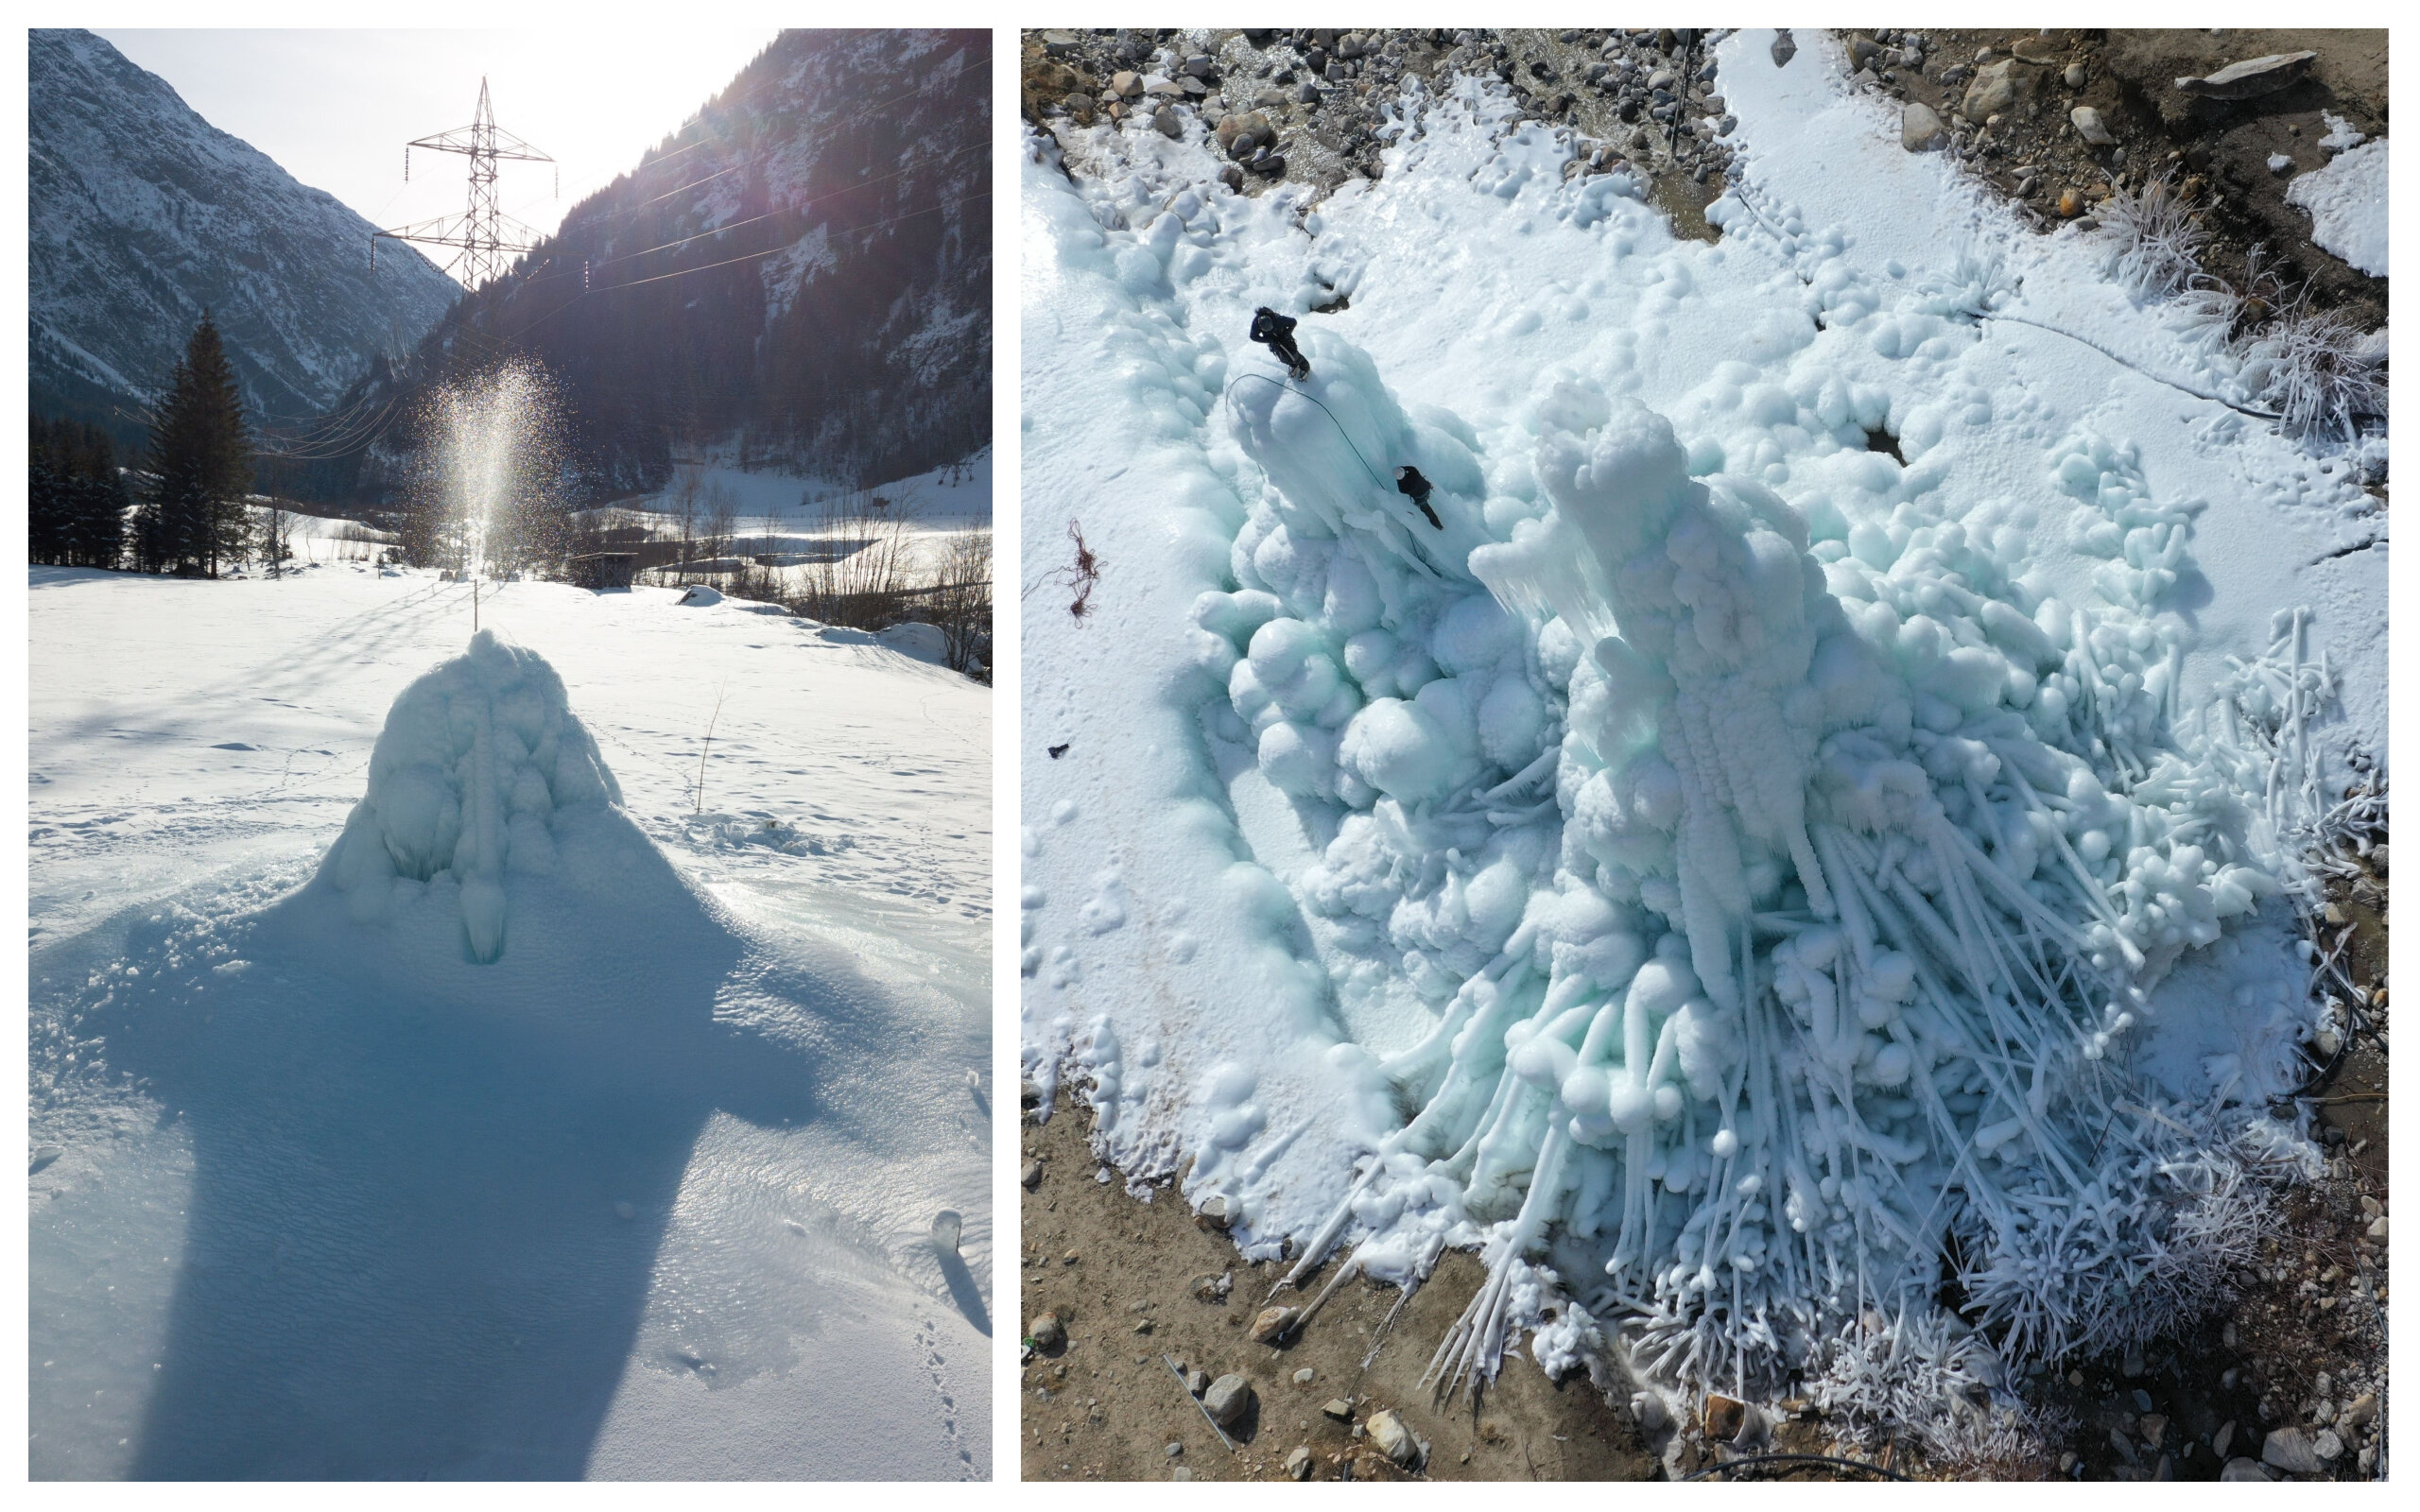
\includegraphics[width=12 cm]{figs/2AIRs.jpg}
	\caption{The Swiss and Indian \ac{AIRs} were 5 $m$ and 13 $m$ tall on January 9 and March 3, 2021 respectively. Picture
		credits: Daniel Bürki (left) and Thinles Norboo (right)}
	\label{fig:2AIRs}
\end{figure}

\subsection{Swiss site}

The Guttannen site (46.66 $\degree$N, 8.29 $\degree$E) is situated in the Berne region, Switzerland and has an
altitude of 1047 $m$ a.s.l. In the winter (Oct-Apr), mean daily minimum and maximum air temperatures vary
between -13 and 15 $\degree C$. Clear skies are rare, averaging around 7 days during winter. Daily winter
precipitation can sometimes be as high as 100 $mm$. These values are based on 30 years of hourly historical
meteorological data series \citep{meteoblueClimateGuttannen2021}. Several \ac{AIRs} were constructed by the Guttannen
Bewegt Association, the University of Fribourg and the Lucerne University of Applied Sciences and Arts during
the winters of 2020-22.

\subsection{Indian site}

The Gangles site (34.22 $\degree$N, 77.61 $\degree$E) is located around 20 km north of Leh city in the Ladakh
region, lying at 4025 $m$ a.s.l.. The mean annual temperature is $5.6 \, \degree C$, and the thermal range is
characterized by high seasonal variation. During January, the coldest month, the mean temperature drops to $-7.2
	\, \degree C$. During August, the warmest month, the mean temperature rises to $17.5 \, \degree C$
\citep{nusserIrrigationDevelopmentUpper2012}. Because of the rain shadow effect of the Himalayan range, the mean
annual precipitation in Leh totals less than 100 $mm$, and there is high interannual variability. While the
average summer rainfall between July and September reaches 37.5 $mm$, the average winter precipitation between
January and March amounts to 27.3 $ mm$ and falls almost entirely as snow. \ac{AIRs} were constructed here by the
Himalayan Institute of Alternatives, Ladakh during the winter of 2020-21.

\subsection{Meteorological data}

Air temperature, relative humidity, wind speed, pressure, longwave and global shortwave radiation are required
as model input.  The resulting dataset highlights the difference in meteorological influences driving ice volume
evolution in the two study sites ( Table \ref{tab:Observations}).

\TODO{Here you have to carefully describe, which meteo series are measured in India and in Switzerland. Please
	give all details here!}

\begin{table}
	\centering
	\caption{Summary of the meteorological observations for \ac{AIRs} built during the respective study period.
		The meteorological measurements are shown using their mean ($\mu$) and standard deviation ($\sigma$) during the study
		period as $\mu \pm \sigma$. }

	\label{tab:Observations}
	\begin{tabular}{|lllll|}
		\hline
		\textbf{Name}        & \textbf{Symbol} & \textbf{IN21} & \textbf{CH21} & \textbf{Units} \\ \hline
		Air temperature      & $T_a    $       & $0 \pm 7$     & $2 \pm 6$     & $\degree C$    \\
		Relative humidity    & $RH     $       & $35 \pm 20$   & $79 \pm 18$   & \%             \\
		Wind speed           & $v_a        $   & $3 \pm 1$     & $2 \pm 2$     & $m/s$          \\
		Direct Shortwave     & $SW_{direct} $  & $246 \pm 333$ & $80 \pm 156$  & $W\,m^{-2}$    \\
		Diffuse Shortwave    & $SW_{diffuse}$  & $0 \pm 0$     & $58 \pm 87$   & $W\,m^{-2}$    \\
		Hourly Precipitation & $ppt        $   & $0 \pm 0$     & $139 \pm 457$ & $mm$           \\
		Pressure             & $p_a         $  & $623 \pm 3$   & $794 \pm 9$   & $hPa$          \\\hline
	\end{tabular}
\end{table}

\TODO{zero is actually not possible then your site is in shadow of a mountain or in morning and evening a quite
	large amount of diffuse shortwave radiation will hit your sensor!}

\subsection{Fountain observations}

The fountain consists of a pipeline and a nozzle. The pipeline has three attributes, namely discharge rate
($Q$), height ($h$) and water temperature ($T_F$). "Discharge rate" represents the discharge rate of the water in
the fountain pipeline. "Height" denotes the height of the fountain pipeline installed. "Fountain water temperature"
is the temperature of water droplets produced by the fountain.

The fountain nozzle has three characteristics, namely the aperture diameter ($dia$) and pressure loss
($P_{nozzle}$). "Pressure loss" denotes the loss of water head due to the fountain nozzle. Additionally,
the observed ice radius formed from the fountain water droplets is denoted as spray radius ($r_F$) (Fig.
\ref{fig:CH20_rad}).

\begin{figure}[htb]
	\centering
	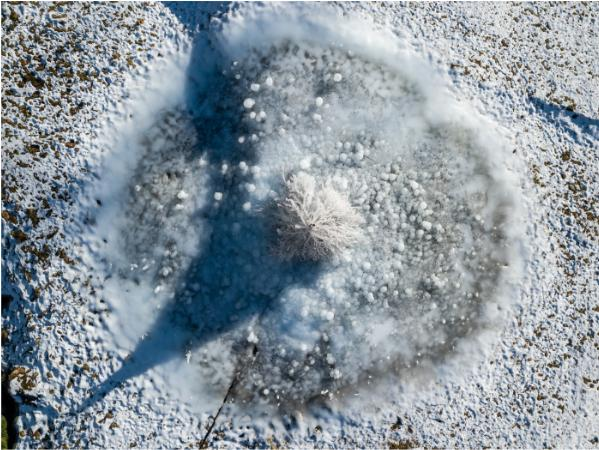
\includegraphics[width=\textwidth/2]{figs/CH20_sprayrad.jpg}
	\caption{Spray radius of the CH20 AIR }
	\label{fig:CH20_rad}
\end{figure}

\subsection{Drone flights}

\begin{table}
	\centering
	\caption{List of all the studied \ac{AIRs}. The study period starts when the fountain was first switched on
		(denoted as Start Date) and ends when the respective AIR either melted or broke into several ice blocks
		(denoted as Expiry Date). }
	\label{tab:AIRs}
	\begin{tabular}{|lllll|}
		\hline
		\textbf{Name}    & \textbf{Start Date} & \textbf{Expiry Date} & \textbf{No. of flights} & \textbf{Spray
		radius}                                                                                                 \\ \hline
		Traditional CH20 & Jan 3 2020          & Apr 6 2020           & 2                       & 7.7 $m$       \\
		Traditional CH21 & Nov 22 2020         & May 10 2021          & 8                       & 6.9 $m$       \\
		Traditional IN21 & Jan 18 2021         & June 20 2021         & 6                       & 10.2 $m$      \\
		Traditional CH22 & Dec 8 2021          & April 12 2022        & 8                       & 4.1 $m$       \\
		Automated CH22   & Dec 8 2021          & April 12 2022        & 6                       & 4.8 $m$       \\ \hline
	\end{tabular}
\end{table}


Several photogrammetric surveys were conducted for each of the \ac{AIRs}. The details of these surveys and the
methodology used to produce the corresponding outputs are explained in paper I. The
\ac{DEMs} generated from the obtained imagery were analysed to document the ice radius, the surface area and the
volume of the ice structures. Ice radius measurements of drone flights which observed either an increase in AIR
circumference or volume were averaged to determine the fountain's spray radius. The number of drone surveys
conducted for each of the AIRs and the corresponding spray radius observed is shown in Table \ref{tab:AIRs}.

\section{Model modules}
\label{sec:modules}

A bulk energy and mass balance model is used to calculate the amounts of ice, meltwater, water vapour and
wastewater of the AIR. In each hourly time step, the model uses the AIR surface area, energy and mass balance
calculations to estimate its ice volume, surface temperature and wastewater as shown in Fig. \ref{fig:schema}.

\begin{figure}
	\begin{center}
		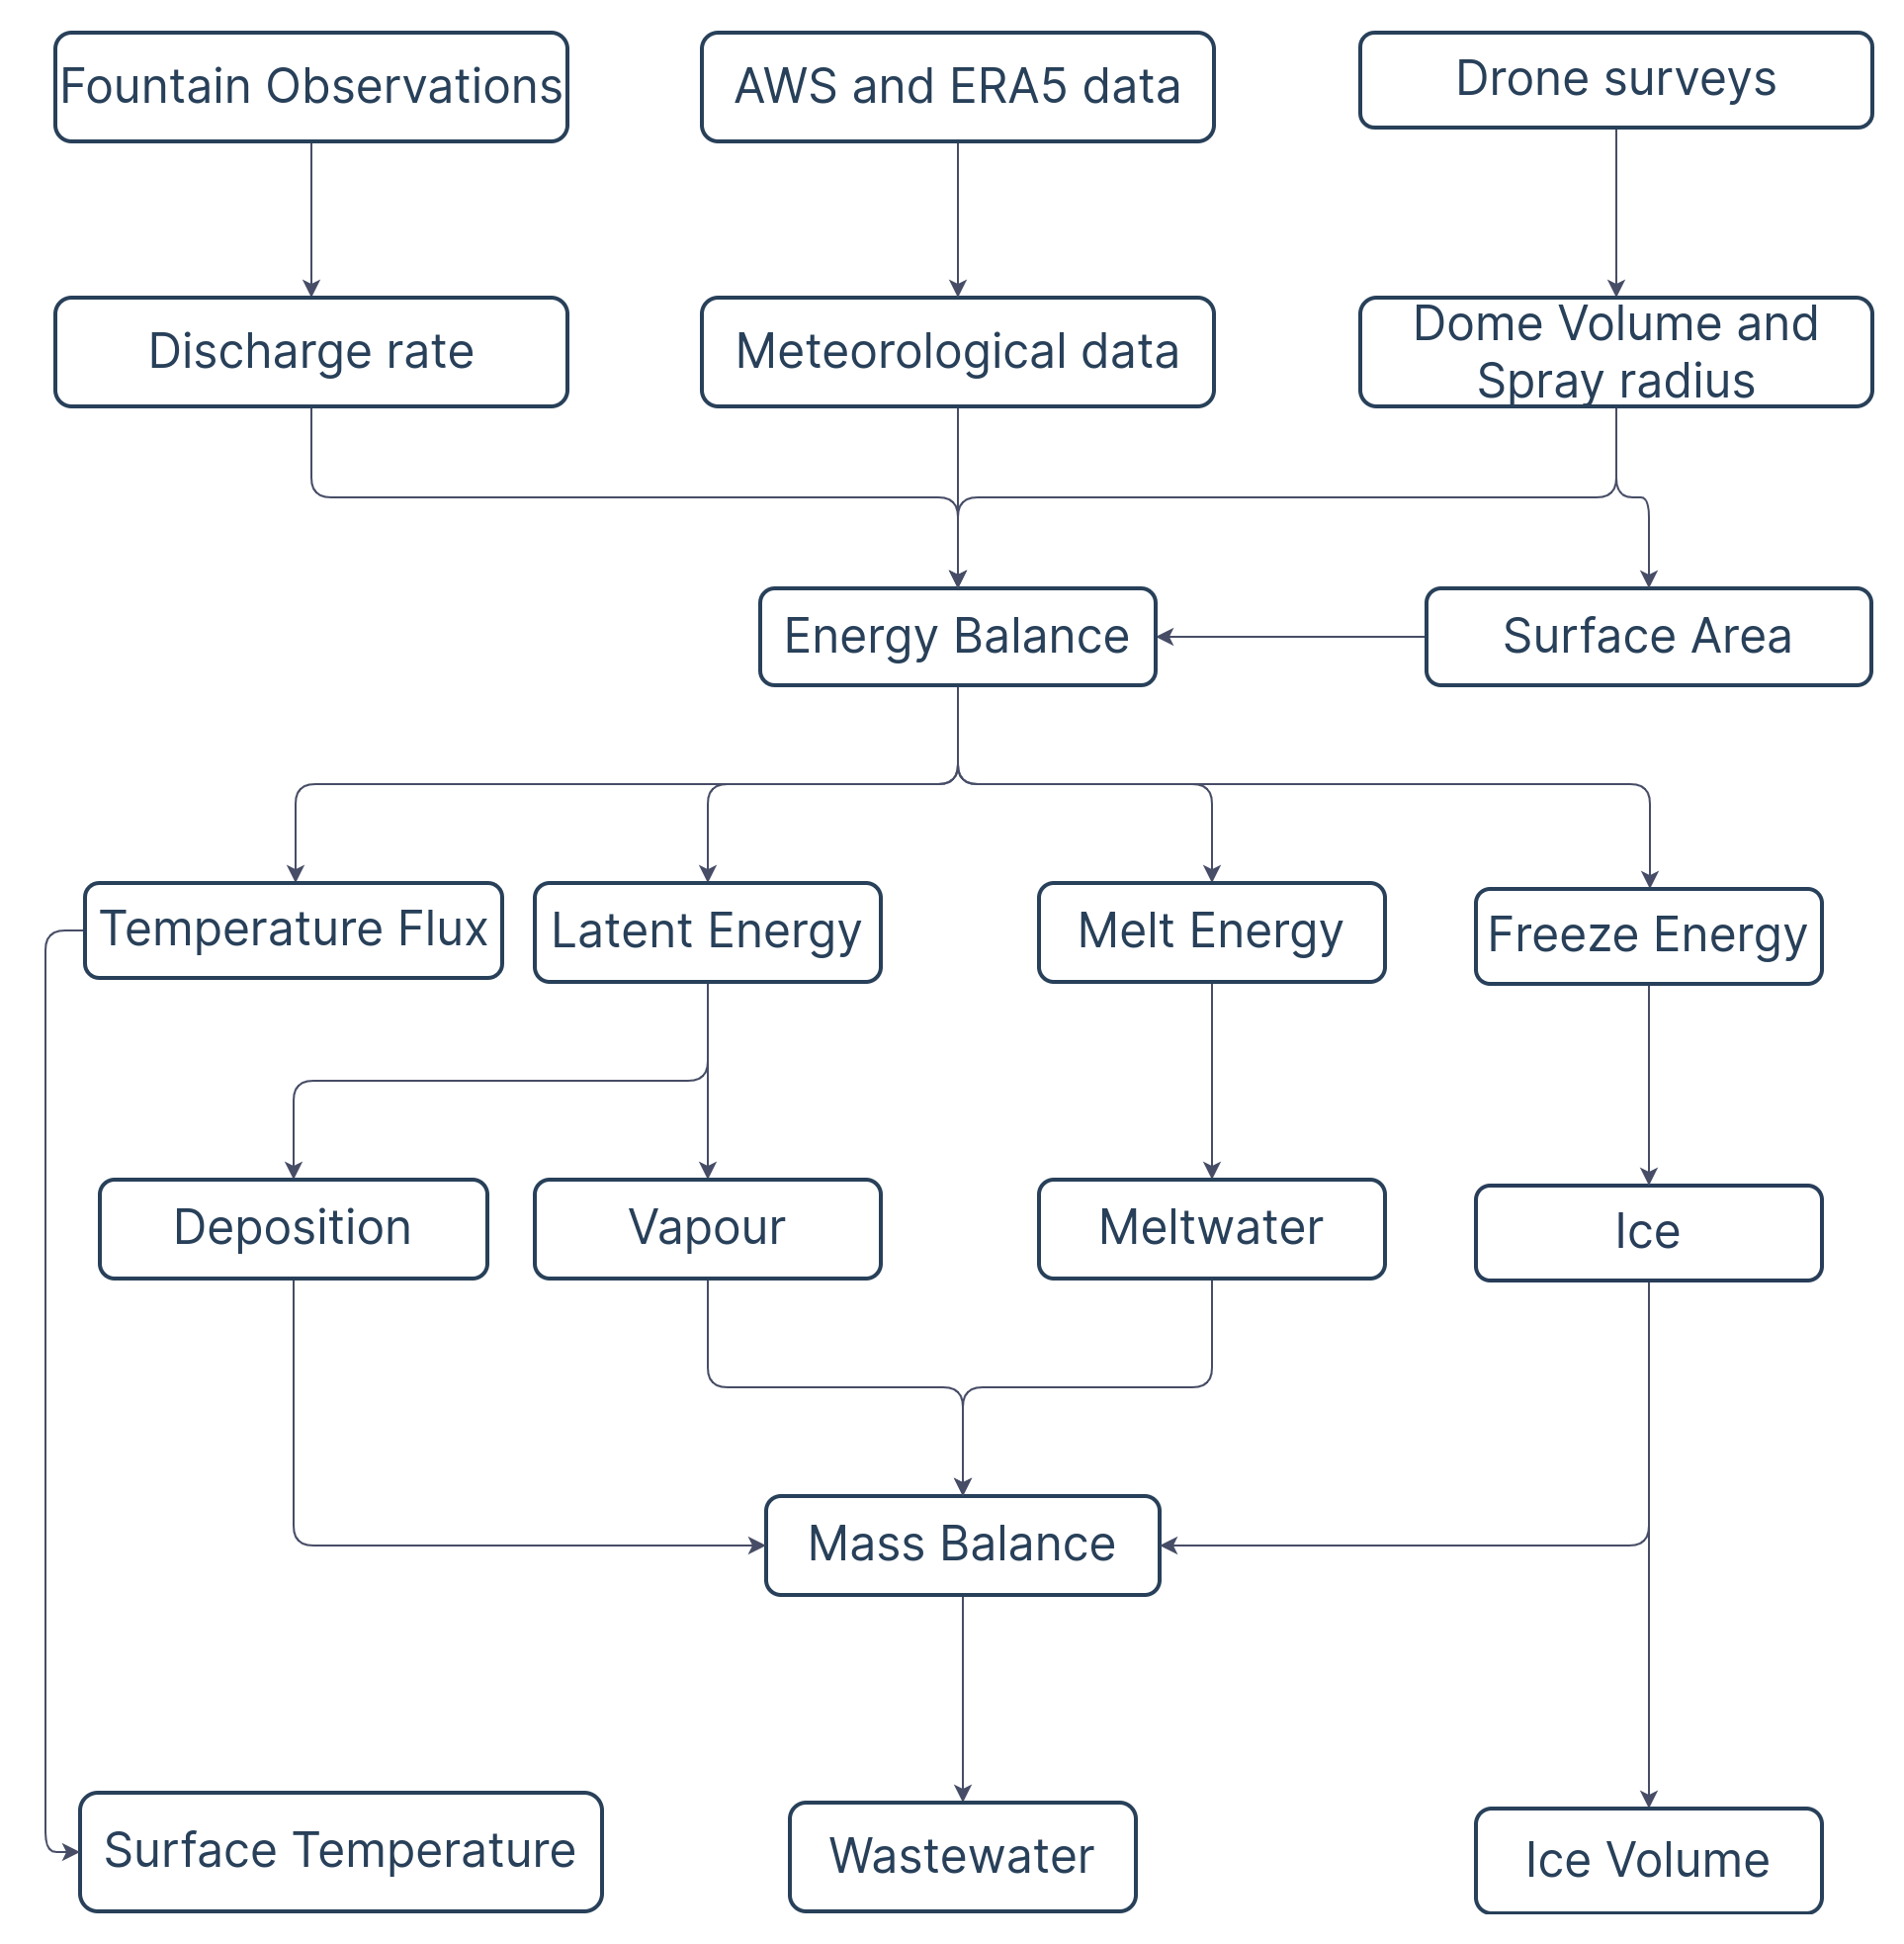
\includegraphics[width=10 cm]{figs/model_schematic.jpg}
	\end{center}
	\caption{Model schematic showing the workflow used in the model at every time step. }
	\label{fig:schema}
\end{figure}

\subsection{Shape evolution module} \label{sec:shape}

The model assumes the AIR shape to be a cone and assigns the following shape attributes:

\begin{subequations}
	\begin{align}
		\label{eq:A}
		A_{cone}^i & = \pi \cdot r_{cone}^i \cdot \sqrt{{(r_{cone}^i)}^2 + {(h_{cone}^i})^ 2} \\
		\label{eq:V}
		V_{cone}^i & = \pi/3 \cdot {(r_{cone}^i)}^2 \cdot h_{cone}^i                          \\
		\label{eq:thickness}
		j_{cone}^i & =\frac{\Delta M_{ice}^i}{\rho_{water}* A_{cone}^i}
	\end{align}
\end{subequations}

where $i$ denotes the model time step, $r_{cone}^i$ is the radius; $h_{cone}^i$ is the height; $A_{cone}^i$ is
the surface area; $V_{cone}^i$ is the volume and $j_{cone}^i$ is the AIR surface normal thickness change as shown
in Fig. \ref{fig:shape}. $M_{ice}^i$ is the mass of the AIR and $\Delta M_{ice}^i = M_{ice}^{i-1} -
	M_{ice}^{i-2}$. Henceforth, the equations used display the model time step superscript $i$ only if it is different
from the current time step.

AIR density can be defined as:

\begin{equation}
	\rho_{cone} = \frac{M_{F} + M_{dep} + M_{ppt}}{(M_{F} + M_{dep})/\rho_{ice} + M_{ppt}/\rho_{snow}}
\end{equation}

where $M_F$ is the cumulative mass of the fountain discharge; $M_{ppt}$ is the cumulative precipitation;
$M_{dep}$ is the cumulative accumulation through water vapour deposition; $\rho_{ice}$ is the ice density (917
$kg\,m^{-3}$) and $\rho_{snow}$ is the density of wet snow (300 $kg\,m^{-3}$) taken from
\cite{cuffeyPhysicsGlaciers2010} .

AIR volume can also be expressed as:

\begin{equation} V_{cone} =\frac{M_{ice}} {\rho_{cone}} \label{eq:V1} \end{equation}

The initial radius of the AIR is assumed to be $r_F$. The initial height $h_0$ depends on the dome volume
$V_{dome}$ used to construct the AIR as follows:

\begin{equation}
	h_{0} =  \Delta x + \frac{3 \cdot V_{dome}}{\pi \cdot (r_F)^2 }
	\label{eq:h0}
\end{equation}

where $\Delta x$ is the surface layer thickness (defined in Section \ref{sec:energy})

During the subsequent time steps, the dimensions of the AIR evolve assuming a uniform thickness change ($j_{cone}$)
across its surface area with an invariant slope $s_{cone} = \frac{h_{cone}}{r_{cone}}$ .  During these time
steps, the volume is parameterised using Eqn. \ref{eq:V} as:

\begin{equation} 
  V_{cone} = \frac{\pi \cdot {(r_{cone})}^3 \cdot s_{cone}}{3} 
\label{eq:V2} 
\end{equation}

We define the ice stupa boundary through its spray radius, i.e. we assume ice formation is negligible when $r_{cone} >
	r_{F}$. Combining Eqns. \ref{eq:V},  \ref{eq:V1}, \ref{eq:h0} and \ref{eq:V2}, the geometric evolution of the
Ice stupa at each time step $i$ can be determined by considering the following rules:

\begin{equation} (r_{cone},\, h_{cone}) = \left\{ \begin{array}{ll} (r_F ,\, h_0)                                                                          & \textit{ if } i=0 \\
             (r_{cone}^{i-1},\, \frac{3 \cdot M_{ice}}{\pi \cdot \rho_{ice} \cdot {(r_{cone}^{i-1})}^2}) & \textit{ if }
             r_{cone}^{i-1} \geq r_{F} \textit{ and } \Delta M_{ice} > 0                                                     \\ (\frac{3 \cdot M_{ice}}{\pi \cdot \rho_{ice} \cdot s_{cone}})^{1/3} \cdot (1,\,  s_{cone}) &
             otherwise\end{array} \right.  \label{eq:A2} \end{equation}

\subsection{Energy balance module} \label{sec:energy}

\begin{figure}
	\begin{center}
		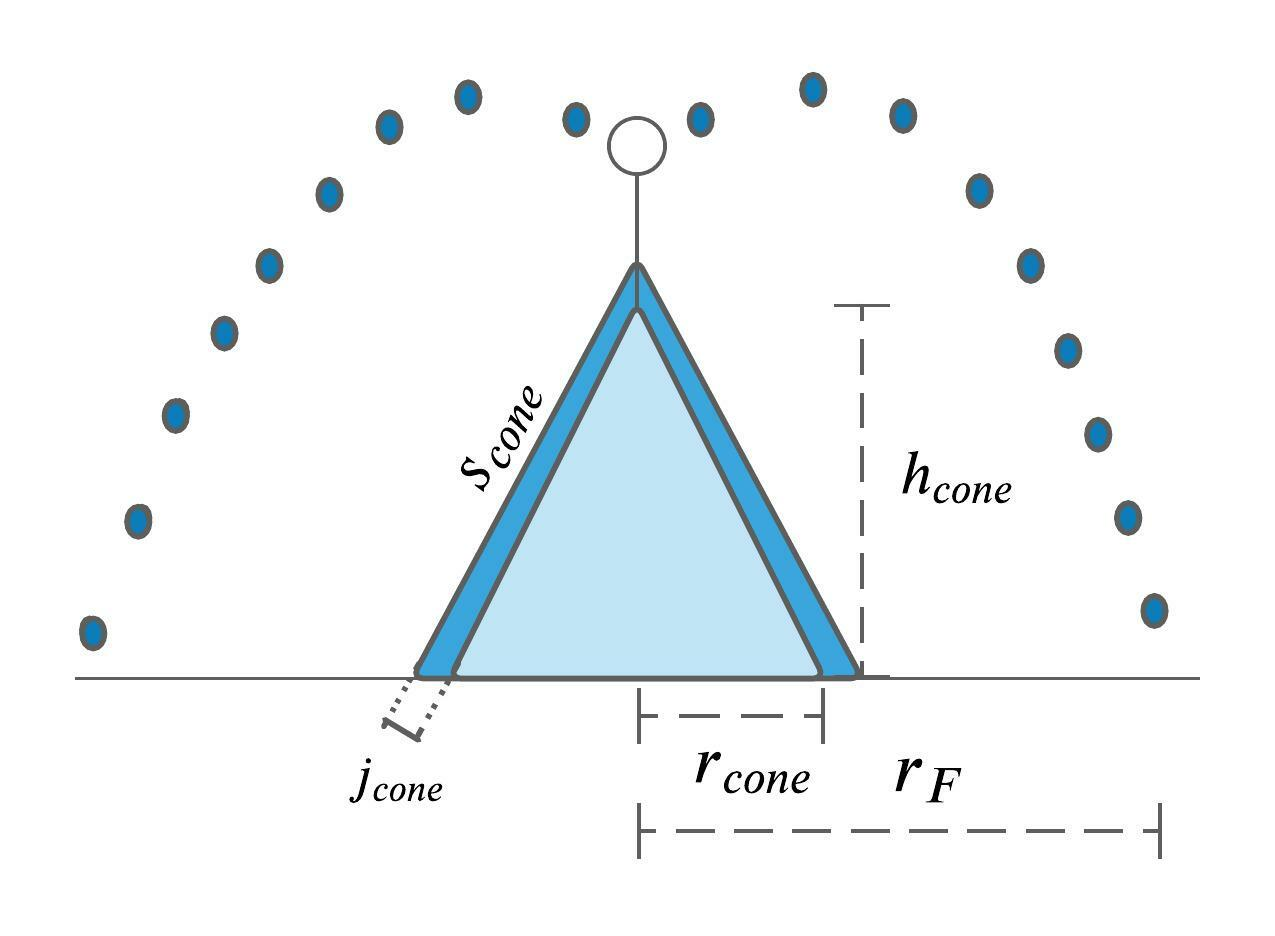
\includegraphics[width=10 cm]{figs/AIR_schematic.jpeg}
	\end{center}
	\caption{Shape variables of the AIR. $r_{cone}$ is the radius, $h_{cone}$ is the height, $j_{cone}$ is the
		thickness change and $s_{cone}$ is the slope of the ice cone. $r_F$ is the spray radius of the fountain.}
	\label{fig:shape}
\end{figure}

We approximate the energy balance at the surface of an AIR by a one-dimensional description of energy fluxes
into and out of a (thin) layer with thickness $\Delta x$:

\begin{equation}
	\rho_{cone} \cdot c_{ice} \cdot \frac{\Delta T}{\Delta t} \cdot \Delta x = q_{SW} + q_{LW} + q_{L} + q_{S} + q_{F}+ q_{R} + q_{G}
	\label{eqn:EB}
\end{equation}

Upward and downward fluxes relative to the ice surface are positive and negative, respectively. The first term
is the energy change of the surface layer, which can be translated into a phase change energy should phase
changes occur. $q_{SW}$ is the net shortwave radiation; $q_{LW}$ is the net longwave radiation; $q_{L}$ and
$q_{S}$ are the turbulent latent and sensible heat fluxes. $q_{F}$ and $q_{R}$ represent the heat exchange of
the fountain water droplets and rain droplets with the AIR ice surface respectively. $q_{G}$ represents ground
heat flux between the AIR surface and its interior.

The energy flux acts upon the AIR surface layer, which has an upper and lower boundary defined by the atmosphere
and the ice body of the AIR, respectively. Here, we define the surface temperature $T_{ice}$ to be the modelled
average temperature of the ice stupa surface layer.

\subsubsection{Net Shortwave Radiation \texorpdfstring{$q_{SW}$}{Lg}} \label{sec:SW}

The net shortwave radiation $q_{SW}$ is computed as follows:

\begin{equation} q_{SW} = (1- \alpha)\cdot (SW_{direct} \cdot f_{cone} + SW_{diffuse}) \label{eqn:SW} \end{equation}

where $SW_{direct}$ and $SW_{diffuse}$ are the direct and diffuse shortwave radiation, $\alpha$ is the
modelled albedo and $f_{cone}$ is the area fraction of the ice structure exposed to the direct shortwave
radiation.

The albedo varies depending on the water source that formed the current AIR surface layer. During the fountain
runtime, the albedo assumes a constant value corresponding to ice albedo. However, after the fountain is
switched off, the albedo can reset to snow albedo during snowfall events and then decay back to ice albedo. We
use the scheme described in \cite{oerlemansYearRecordGlobal1998} to model this process. The scheme records the
decay of albedo with time after fresh snow is deposited on the surface. $\delta t$ records the number of time
steps after the last snowfall event. After snowfall, albedo changes over a time step, $\delta t$ , as

\begin{equation} \alpha=\alpha_{ice}+(\alpha_{snow}-\alpha_{ice}) \cdot e^{(-\delta t)/\tau} \label{eqn:alb}
\end{equation}

where $\alpha_{ice}$ is the bare ice albedo value (0.25), $\alpha_{snow}$ is the fresh snow albedo value (0.85)
and $\tau$ is a decay rate (16 $days$), which determines how fast the albedo of the ageing snow recedes back to
ice albedo. Discharge events decrease the decay rate by a factor of $\alpha_{ice}/\alpha_{snow}$.

The solar area fraction $f_{cone}$ of the ice structure exposed to the direct shortwave radiation depends on the shape
considered. Using the solar elevation angle $\theta_{sun}$, the solar beam can be considered to have a vertical
component, impinging on the horizontal surface (semicircular base of the AIR), and a horizontal component
impinging on the vertical cross section (a triangle). The solar elevation angle $\theta_{sun}$ used is modelled
using the parametrization proposed by \cite{woolfComputationSolarElevation1968}. Accordingly, $f_{cone}$ is determined as follows:

\begin{equation}
	\begin{split}
		f_{cone}& =\frac{(0.5 \cdot r_{cone} \cdot h_{cone}) \cdot cos \theta_{sun} +(\pi \cdot
		{(r_{cone})}^2/2) \cdot sin \theta_{sun} }{\pi \cdot r_{cone} \cdot ({(r_{cone})}^2+{(h_{cone})}^2)^{1/2}}\\
	\end{split}
	\label{eqn:f_{cone} }
\end{equation}

The diffuse shortwave radiation is assumed to impact the conical AIR surface uniformly.

\subsubsection{Net Longwave Radiation \texorpdfstring{$q_{LW}$}{Lg}} \label{sec:LW}

The net longwave radiation $q_{LW}$ is determined as follows:

\begin{equation}
	q_{LW}= LW_{in}-\sigma \cdot \epsilon_{ice} \cdot {(T_{ice}+ 273.15)}^4
	\label{eqn:LW}
\end{equation}

where $T_{ice}$ is the modelled surface temperature given in [$\degree C$],
$\sigma=5.67\cdot10^{-8}\,Jm^{-2}s^{-1}K^{-4}$ is the Stefan-Boltzmann constant, $LW_{in}$ denotes the incoming
longwave radiation and $\epsilon_{ice}$ is the corresponding emissivity value for the ice stupa surface (0.97).

The incoming longwave radiation $LW_{in}$ for the Indian site, where no direct measurements were available, is
determined as follows:

\begin{equation}
	LW_{in}=\sigma \cdot \epsilon_a \cdot {(T_a+ 273.15)}^4
	\label{eqn:LWin}
\end{equation}

here $T_a$ represents the measured air temperature and $\epsilon_a$ denotes the atmospheric emissivity. We
approximate the atmospheric emissivity $\epsilon_a$ using the equation suggested by \cite{brutsaertEvaporationAtmosphereTheory1982},
considering air temperature and vapor pressure (Eqn.  \ref{eqn:atm_e}). The vapor pressure of air over water and
ice was obtained using Eqn. \ref{eqn:vp}.  The expression defined in \cite{brutsaertDerivableFormulaLongwave1975} for clear skies
(first term in equation \ref{eqn:atm_e}) is extended with the correction for cloudy skies after
\cite{brutsaertEvaporationAtmosphereTheory1982} as follows:

\begin{equation}
	\epsilon_a=1.24 \cdot (\frac{p_{v,w}}{(T_a+273.15)})^{1/7}\cdot(1+0.22\cdot{cld}^2) \label{eqn:atm_e}
\end{equation}

with a cloudiness index $cld$, ranging from 0 for clear skies to 1 for complete overcast skies. For the Indian
site, we assume cloudiness to be negligible.

\subsubsection{Turbulent fluxes} \label{sec:Qs}

The turbulent sensible $q_{S}$ and latent heat $q_{L}$ fluxes are computed with the following expressions
proposed by \cite{garrattAtmosphericBoundaryLayer1992}:

\begin{equation}
	q_{S}=\mu_{cone}\cdot c_{a} \cdot \rho_{a} \cdot p_{a}/p_{0,a} \cdot \frac{\kappa^2 \cdot v_a \cdot
		(T_a-T_{ice})}{{(\ln{\frac{h_{AWS}}{z_{0}}})}^2}
	\label{eqn:qs}
\end{equation}

\begin{equation}
	q_{L}=\mu_{cone}\cdot 0.623 \cdot L_s \cdot \rho_{a}/p_{0,a} \cdot \frac{\kappa^2 \cdot
	v_a(p_{v,w}-p_{v,ice})}{{(\ln{\frac{h_{AWS}}{z_{0}}})}^2}
\end{equation}

where $h_{AWS}$ is the measurement height above the ground surface of the \ac{AWS} (around $2\,m$ for all sites),
$v_a$ is the wind speed in [$m\,s^{-1}$], $c_a$ is the specific heat of air at constant pressure (1010 J
$kg^{-1} K^{-1}$), $\rho_{a}$ is the air density at standard sea level (1.29 $kg m^{-3}$), $p_{0,a}$ is the air
pressure at standard sea level (1013 $hPa$), $p_{a}$ is the measured air pressure, $\kappa$ is the von Karman
constant (0.4), $z_{0}$ is the surface roughness (3 $mm$) and $L_s$ is the heat of sublimation (2848
$kJ\,kg^{-1}$). The vapor pressure of air with respect to water ($p_{v,w}$) and with respect to ice
($p_{v,ice}$) was obtained using the formulation given in \cite{huangSimpleAccurateFormula2018} :

\begin{equation}
	\begin{split}
		p_{v,w}&=e^{\frac{(34.494 - \frac{4924.99}{T_{a} + 237.1})}{(T_a + 105)^{1.57} \cdot 100}} \cdot \frac{RH}{100} \\
		p_{v,ice}&=e^{\frac{(43.494 - \frac{6545.89}{T_{ice} + 278})}{(T_{ice} + 868)^{2} \cdot 100}} \\
	\end{split} \label{eqn:vp}
\end{equation}

The dimensionless parameter $\mu_{cone}$ is an exposure parameter that deals with the fact that AIR has a rough
appearance and forms an obstacle to the wind regime. This factor accounts for the larger turbulent fluxes due to
the roughness of the surface \citep{oerlemansBriefCommunicationGrowth2021}, and is a function of the AIR slope
as follows:

\begin{equation}
	\mu_{cone} = 1 + \frac{s_{cone}}{2}
	\label{eqn:mu}
\end{equation}

A possible source of error is the fact that wind measurements from the horizontal plane at the \ac{AWS} are used,
which might be different from those on a slope. However, without detailed data sets from the AIR surface, we
retain this assumption.

\subsubsection{Fountain discharge heat flux \texorpdfstring{$q_{F}$}{Lg} } \label{sec:heatflux}

The fountain water temperature $T_F$ is assumed to cool to 0 $\degree C$ after contact with the ice surface.
$T_F$ is equal to the measured source water temperature. But during time periods when the ambient temperature is
subzero, $T_F$ is assumed to be 0 $\degree C$. Thus, the heat flux caused by this process is:

\begin{equation}
	q_{F} = \left\{ \begin{array}{ll}
		\frac{ \Delta M_F \cdot c_{water} \cdot T_F}{\Delta t \cdot A_{cone}} & \textit{ if } T_{temp} > 0 \\
		0                                                                     & \textit{ otherwise}
	\end{array} \right.
\end{equation}

with $c_{water}$ as the specific heat of water (4186 J $kg^{-1} K^{-1}$).

\subsubsection{Rain heat flux \texorpdfstring{$q_{R}$}{Lg} }

The influence of rain events on the albedo and on the ice stupa's energy balance was assumed to be similar to that of discharge
events. However, the water temperature of a rain event was assumed to be equal to the air temperature. Accordingly,
the heat flux generated due to a rain event was determined:

\begin{equation}
	q_{R} = \frac{ \Delta M_{ppt} \cdot c_{water} \cdot T_a}{\Delta t \cdot A_{cone}}
	\label{eqn:qR}
\end{equation}

\subsubsection{Bulk ice stupa heat flux \texorpdfstring{$q_{G}$}{Lg}} \label{sec:Bulkflux}

The bulk ice stupa heat flux $q_{G}$ corresponds to the ground heat flux in normal soils and is caused by the
temperature gradient between the surface layer ($T_{ice}$) and the ice body ($T_{bulk}$). It is expressed by
using the heat conduction equation as follows:

\begin{equation} q_{G} = k_{ice} \cdot (T_{bulk}-T_{ice}^{i-1})/l_{cone} \label{eqn:qG}    \end{equation}

where $k_{ice}$ is the thermal conductivity of ice (2.123 $W\, m^{-1}\,K^{-1}$) , $T_{bulk}$ is the mean
temperature of the ice body within the ice stupa and $l_{cone}$ is the average distance of any point in the
surface to any other point in the ice body. $T_{bulk}$ is initialised as 0 $\degree C$ and later determined from
Eqn. \ref{eqn:qG} as follows:

\begin{equation} T_{bulk}^{i+1} = T_{bulk} - (q_{G} \cdot A \cdot \Delta t)/(M_{ice} \cdot c_{ice}) \end{equation}

Since \ac{AIRs} typically have conical shapes with $r_{cone} > h_{cone}$, we assume that the center of mass of the cone
body is near the base of the fountain. Thus, the distance of every point in the AIR surface layer from the cone
body's center of mass is between $h_{cone}$ and $r_{cone}$. Therefore, we calculate $q_{G}$ assuming $l_{cone} = (r_{cone} +
	h_{cone})/2$.

\subsubsection{Phase changes}\label{sec:phase}

This section explains the numerical procedures to model phase changes at the surface layer. Let
$T_{temp}$ be the calculated surface temperature. Therefore, Eqn. \ref{eqn:EB} can be rewritten as:

$$q_{total} =\rho_{ice} \cdot c_{ice} \cdot \frac{(T_{temp}-T_{ice})}{\Delta t} \cdot \Delta x$$

where $q_{total}$ represents the total energy available to be redistributed. Even if the numerical heat transfer
solution produces temperatures which are $T_{temp}>0\, \degree C$, say from intense shortwave radiation, the ice
temperature must remain at $T_{temp} = 0\, \degree C$. The ‘‘excess’’ energy is used to drive the melting
process. Moreover, the energy input is used to melt the surface ice layer, and not to raise the surface
temperature to some unphysical value. Similarly, for freezing to occur, three conditions are required. Firstly,
fountain water is present ($\Delta M_{F} > 0 $) and secondly the calculated temperature of the ice, $T_{temp}$,
is below $0\, \degree C$. However, these two conditions are not sufficient as the latent heat turbulent fluxes
can only contribute to temperature fluctuations. Therefore, an additional condition, namely, $(q_{total}-q_{L})
	< 0$, is required. Depending on the above conditions, the total energy $q_{total}$ can be redistributed
for the melting ($q_{melt}$), freezing ($q_{freeze}$) and surface temperature change ($q_{T}$) processes as
follows:

\begin{equation}
	q_{total} = \left\{ \begin{array}{ll}
		q_{freeze} + q_{T} & \textit{ if } \Delta M_{F} > 0 \textit{ and } T_{temp} < 0 \textit{ and }(q_{total}-q_{L}) < 0 \\
		q_{melt} + q_{T}   & \textit{ otherwise}
	\end{array} \right.
\end{equation}

Henceforth, time steps when the the total energy is redistributed to the freezing energy are called freezing
events and the rest of the time steps are called melting events.


During a freezing event, the AIR surface is assumed to warm to $0 \degree C$. The available energy
$(q_{total}-q_{L})$ is further increased due to this change in surface temperature represented by the energy
flux:

$$q_{0} = \frac{\rho_{ice} \cdot \Delta x \cdot c_{ice} \cdot T_{ice}^{i-1}}{\Delta t}$$

The available fountain discharge ($\Delta M_{F}$) may not be sufficient to utilize all the freezing energy. At such times,
the additional freezing energy further cools down the surface temperature. Accordingly, the surface energy flux
distribution during a freezing event can be represented as:

\begin{equation}
	(q_{freeze}, q_{T}) = \left\{ \begin{array}{ll}
		(\frac{\Delta M_{F} \cdot L_f
		}{A_{cone} \cdot \Delta t}
		, q_{total}+\frac{\Delta M_{F} \cdot L_f
		}{A_{cone} \cdot \Delta t})          & \textit{ if  } \Delta M_{F} \textit{ insufficient } \\
		(q_{total}-q_{L}+q_{0}, q_{L}-q_{0}) & \textit{ otherwise }                                \\
	\end{array} \right.
\end{equation}

If $T_{temp} > 0 \degree C$, then energy is reallocated from $q_{T}$ to $q_{melt}$ to maintain surface
temperature at melting point. The total energy flux distribution during a melting event can be represented as:

\begin{equation}
	(q_{melt}, q_{T}) = \left\{ \begin{array}{ll}
		(0, q_{total})
		                                                                                                                                                               & \textit{ if } T_{temp} \leq 0 \\
		(\frac{T_{temp} \cdot \rho_{ice} \cdot c_{ice} \cdot \Delta x}{\Delta t}, q_{total}-\frac{T_{temp} \cdot \rho_{ice} \cdot c_{ice} \cdot \Delta x}{\Delta t}  ) & \textit{ if } T_{temp} > 0
	\end{array} \right.
\end{equation}

\subsection{Mass balance module}

The mass balance equation for an AIR is represented as:

\begin{equation}
	\frac{\Delta M_{F} + \Delta M_{ppt} + \Delta M_{dep}}{\Delta t} = \frac{\Delta M_{ice} +\Delta M_{water} +
		\Delta M_{sub} + \Delta M_{waste}}{\Delta t}  \\
	\label{eq:MB}
\end{equation}

where $M_{F}$ is the cumulative mass of the fountain discharge; $M_{ppt}$ is the cumulative precipitation;  $M_{dep}$ is the cumulative
accumulation through water vapour deposition; $M_{ice}$ is the cumulative mass of ice; $M_{water}$ is the cumulative
mass of melt water; $M_{sub}$ represents the cumulative water vapor loss by sublimation and $M_{waste}$ represents the
fountain wastewater that did not interact with the AIR. The left hand side of equation \ref{eq:MB} represents the rate of
mass input and the right hand side represents the rate of mass output for an AIR.

Precipitation input is calculated as shown in equation \ref{eq:ppt} where $\rho_{w}$ is the density of water (1000
$kg\,m^{-3}$), $\Delta ppt/ \Delta t$ is the measured precipitation rate in [$m\,s^{-1}$] and $T_{ppt}$ is the temperature threshold
below which precipitation falls as snow. Here, snowfall events were identified using $T_{ppt}$ as $1 \degree C$. Snow
mass input is calculated by assuming a uniform deposition over the entire circular footprint of the AIR.

The latent heat flux is used to estimate either the evaporation and condensation processes or sublimation and deposition
processes as shown in equation \ref{eq:vap}. During the time steps at which the surface temperature is below 0 $\degree C$ only
sublimation and deposition can occur, but if the surface temperature reaches 0 $\degree C$, evaporation and condensation
can also occur. As the differentiation between evaporation and sublimation (and condensation and deposition) when the
air temperature reaches 0 $\degree C$ is challenging, we assume that negative (positive) latent heat fluxes correspond
only to sublimation (deposition), i.e. no evaporation (condensation) is calculated.

Since we have categorized every time step as a freezing or melting event, we can determine the melting/freezing
rates and the corresponding meltwater/ice quantities as shown in equations \ref{eq:m_freeze/melt}, \ref{eq:mwat}
and \ref{eq:mcone}. Having calculated all other mass components, the fountain wastewater generated every
time step can be calculated using Eqn. \ref{eq:MB}.

\begin{subequations}
	\begin{align}
		\frac{\Delta M_{F}}{\Delta t}                                      & = \left\{ \begin{array}{ll} \frac{60}{\rho_w \cdot \Delta t} \cdot d_F
			 & \textit{ if fountain is on} \\ 0 & \textit{ otherwise } \\\end{array} \right.                                             \\
		\label{eq:ppt}
		\frac{\Delta M_{ppt}}{\Delta t}                                    & = \left\{ \begin{array}{ll} \pi \cdot
			{(r_{cone})}^2 \cdot
			\rho_{w}\cdot \frac {\Delta ppt}{\Delta t} & \textit{ if } T_{a} < T_{ppt} \\ 0 & \textit{ if } T_{a} \geq T_{ppt} \\\end{array} \right.                                             \\
		\label{eq:vap}
		(\frac{\Delta M_{dep}}{\Delta t}, \frac{\Delta M_{sub}}{\Delta t}) & = \left\{ \begin{array}{ll} \frac{q_{L}
			\cdot A_{cone}}{L_s}\cdot (1,0)  & \textit{ if } q_{L} \geq 0 \\ \frac{q_{L}
			\cdot A_{cone}}{L_s}\cdot (0,-1) & \textit{ if } q_{L} < 0    \\\end{array} \right.                                             \\
		\label{eq:mwat}
		\frac{\Delta M_{water}}{\Delta t}                                  & = \frac{q_{melt} \cdot A_{cone} }{L_f}                                                   \\
		\label{eq:m_freeze/melt}
		\frac{\Delta M_{freeze/melt}}{\Delta t}                            & = \frac{q_{freeze/melt} \cdot A_{cone} }{L_f}                                            \\
		\label{eq:mcone}
		\frac{\Delta M_{ice}}{\Delta t}                                    & = \frac{q_{freeze}\cdot A_{cone} }{L_f} + \frac{\Delta M_{ppt}}{\Delta t} + \frac{\Delta
			M_{dep}}{\Delta t}- \frac{\Delta M_{sub}}{\Delta t}- \frac{\Delta M_{water}}{\Delta t}
	\end{align}
\end{subequations}

Considering \ac{AIRs} as water reservoirs, their net water loss can be defined as:

\begin{equation} \textit{Net water losses} = \frac{M_{waste}+M_{sub}}{(M_F+M_{ppt}+M_{dep})} \cdot 100 \end{equation}

\section{Overview of different models}
\label{sec:MIP}

The model modules described above where used in three different models with varying degree of complexity as
shown in Table \ref{tab:MIP}. The Oerlemans model is the simplest, implemented in just one page of code whereas
the COSISTUPA model is the most complex maintained by a community of modellers. Below we describe the motivation
involved in developing each of these models.

\begin{table}[ht]
	\centering
  \caption{Characteristics of the models used in the estimation of AIR volumes. The models are referred to by
  the short name given in the first row. Full model documentation is given in the original literature (marked in
  italic). }      

	\label{tab:MIP}
	\begin{tabular}{|llll|}
		\hline
		\textbf{Module}        & \textbf{Oerlemans} & \textbf{AIR} & \textbf{COSISTUPA}     \\ 
		\textit{Documentation} & \textit{Paper III} & \textit{Paper I} & \textit{\citet{sauterCOSIPYV1Opensource2020}} \\ 
		                       &                    &                  & \textit{and Section \ref{sec:Cosistupa}}     \\ \hline
		Shape evolution        & Constant radius     & Derived from  & Derived from        \\
                           & or slope            & energy balance & surface mass balance        \\\hline
		Density and temperature& None & 1-dimensional   & 2-dimensional   \\
		variation              &           &        & \\ \hline
	\end{tabular}
\end{table}

\subsection{Oerlemans model}

The objective of the Oerlemans model was to integrate a shape evolution module with glacial models to obtain
first-order estimates of growth and decay rates under various conditions. This model was designed to
qualitatively assess the effects of snow cover, different starting dates, differences between warm and cold
winters, etc. It simulated ice stupa evolution using data from field measurements in Oberengadin region,
Switzerland. 

However, this model was not ideal for comparing between simulated and observed ice stupa volumes. This was
because the model considers the ice stupa to be a single unit with a surface temperature close to the melting
point. This assumption limits the quantification of surface processes which depend strongly on surface
temperature variations. Moreover, the model assumes unlimited water availability which is often not the case
during AIR construction. Also, the model uses a simplistic shape evolution module that ignores the dependence of
shape variables with fountain characteristics. These shortcomings made it necessary to extend the Oerlemans
model further.

\subsection{AIR model}

The AIR model was designed to obtain better validation with measured ice stupa volumes than the Oerlemans model.
In order to do this, it incorporated all the mass and energy balance modules described in Section
\ref{sec:modules} and simulated AIR evolution using data from field measurements in Gangles, India and
Guttannen, Switzerland. The model was calibrated and validated with ice volume and surface area observations
obtained via drone surveys. We calculated the freezing and melting rates for each of the three AIRs and
explained their corresponding magnitudes in terms of the influence of the chosen location and the fountain used.
The model was successful in reproducing the observed ice volume evolution with a correlation greater than 0.96
and an \ac{RMSE} less than 18 \% of the maximum ice volume for three AIRs (Paper I). 

However, the model is not expected to perform well for locations where it has not been calibrated in advance.
Specifically, the surface layer thickness parameter requires prior calibration for better model performance.

\subsection{COSISTUPA: COSIPY + AIR model}
\label{sec:Cosistupa}

In order to reduce the calibration requirements for the AIR model, we combine the AIR model with the COupled
Snowpack and Ice surface energy and mass balance model in PYthon (COSIPY). COSIPY is typically used for
modelling distributed snow and glacier mass changes \citep{sauterCOSIPYV1Opensource2020}. However, it has a
flexible, user-friendly and modular framework allowing it to be an ideal platform to implement the alternate
modules required for modelling ice reservoirs. This modified COSIPY model will be referred to as COSISTUPA model
henceforth.

\subsubsection{Model configuration}

In this section, we describe the main adjustments needed to convert COSIPY modules into the COSISTUPA
model.

The COSIPY model input was extended to include discharge rate and cloudiness index measurements. Additionally,
spray radius parameter was provided as input during model initialization. The model initialization of the ice
cone dimensions were made identical to the AIR model.

Several parametrizations are available for estimating each of the surface processes in COSIPY. Most of the ones
used in the AIR model are among the available options. Additionally, new parametrizations were required to
estimate the conical shape evolution and model the freezing process due to the fountain discharge events. To
extend COSIPY into COSISTUPA, parametrizations of the following processes were modified:

\begin{itemize}

	\item \textbf{Fountain rain heat flux} : The heat flux generated due to the difference in fountain water droplet
	      temperature and surface temperature was introduced as a new energy balance component. This implementation is
	      identical to the selected approach described in Sec. \ref{sec:heatflux}

	\item \textbf{Turbulent flux scaling} : The sensible and the latent heat fluxes were scaled by the $\mu_{cone}$ factor
	      introduced in Sec. \ref{sec:Qs}

	\item \textbf{Freezing process} : Phase transition processes were introduced during time periods when the fountain
	      discharge was active. These processes created new ice layers whenever the energy balance allowed it
	      following the algorithm introduced in Sec. \ref{sec:phase}

	\item \textbf{Conical shape evolution} : The surface mass balance estimation was converted to the volume estimation
	      through the methodology introduced in Sec. \ref{sec:shape}

\end{itemize}

Please note the above list of changes are not exhaustive and represent only the major modifications necessary to
develop the COSISTUPA model.

\subsubsection{Advantages of the COSISTUPA model}

The COSISTUPA model has a modular structure allowing the exchange of routines or parametrizations of physical
processes with little effort for the user. The framework consists of a computational kernel, forming
the runtime environment and taking care of the initialization, the input-output routines, and the
parallelization, as well as the grid and data structures. This structure offers maximum flexibility without
having to worry about the internal numerical flow. The adaptive subsurface scheme allows an efficient and fast
calculation of the otherwise computationally demanding fundamental equations. The surface energy balance scheme
uses established standard parametrizations for radiation as well as for the energy exchange between the
atmosphere and surface. The schemes are coupled by solving both surface energy balance and subsurface fluxes
iteratively in which consistent skin temperature is returned at the interface. COSISTUPA uses a one-dimensional
approach limited to the vertical fluxes of energy and matter but neglects any lateral processes. Accordingly,
the model can be easily set up in parallel computational environments for calculating both energy balance and
climatic surface mass balance of multiple \ac{AIRs} based on flexible horizontal grids and with varying temporal
resolution.

The \ac{RMSE} error of the 5 ice stupas studied in this thesis were within 20 \% of their maximum ice volumes for both
the models (Fig. \ref{fig:Cosistupa}).  However, the COSISTUPA model was 3 times slower than the AIR model. This
is likely due to the additional effort required to resolve the ice temperature spatially.

\begin{figure}[t]
	\centering
	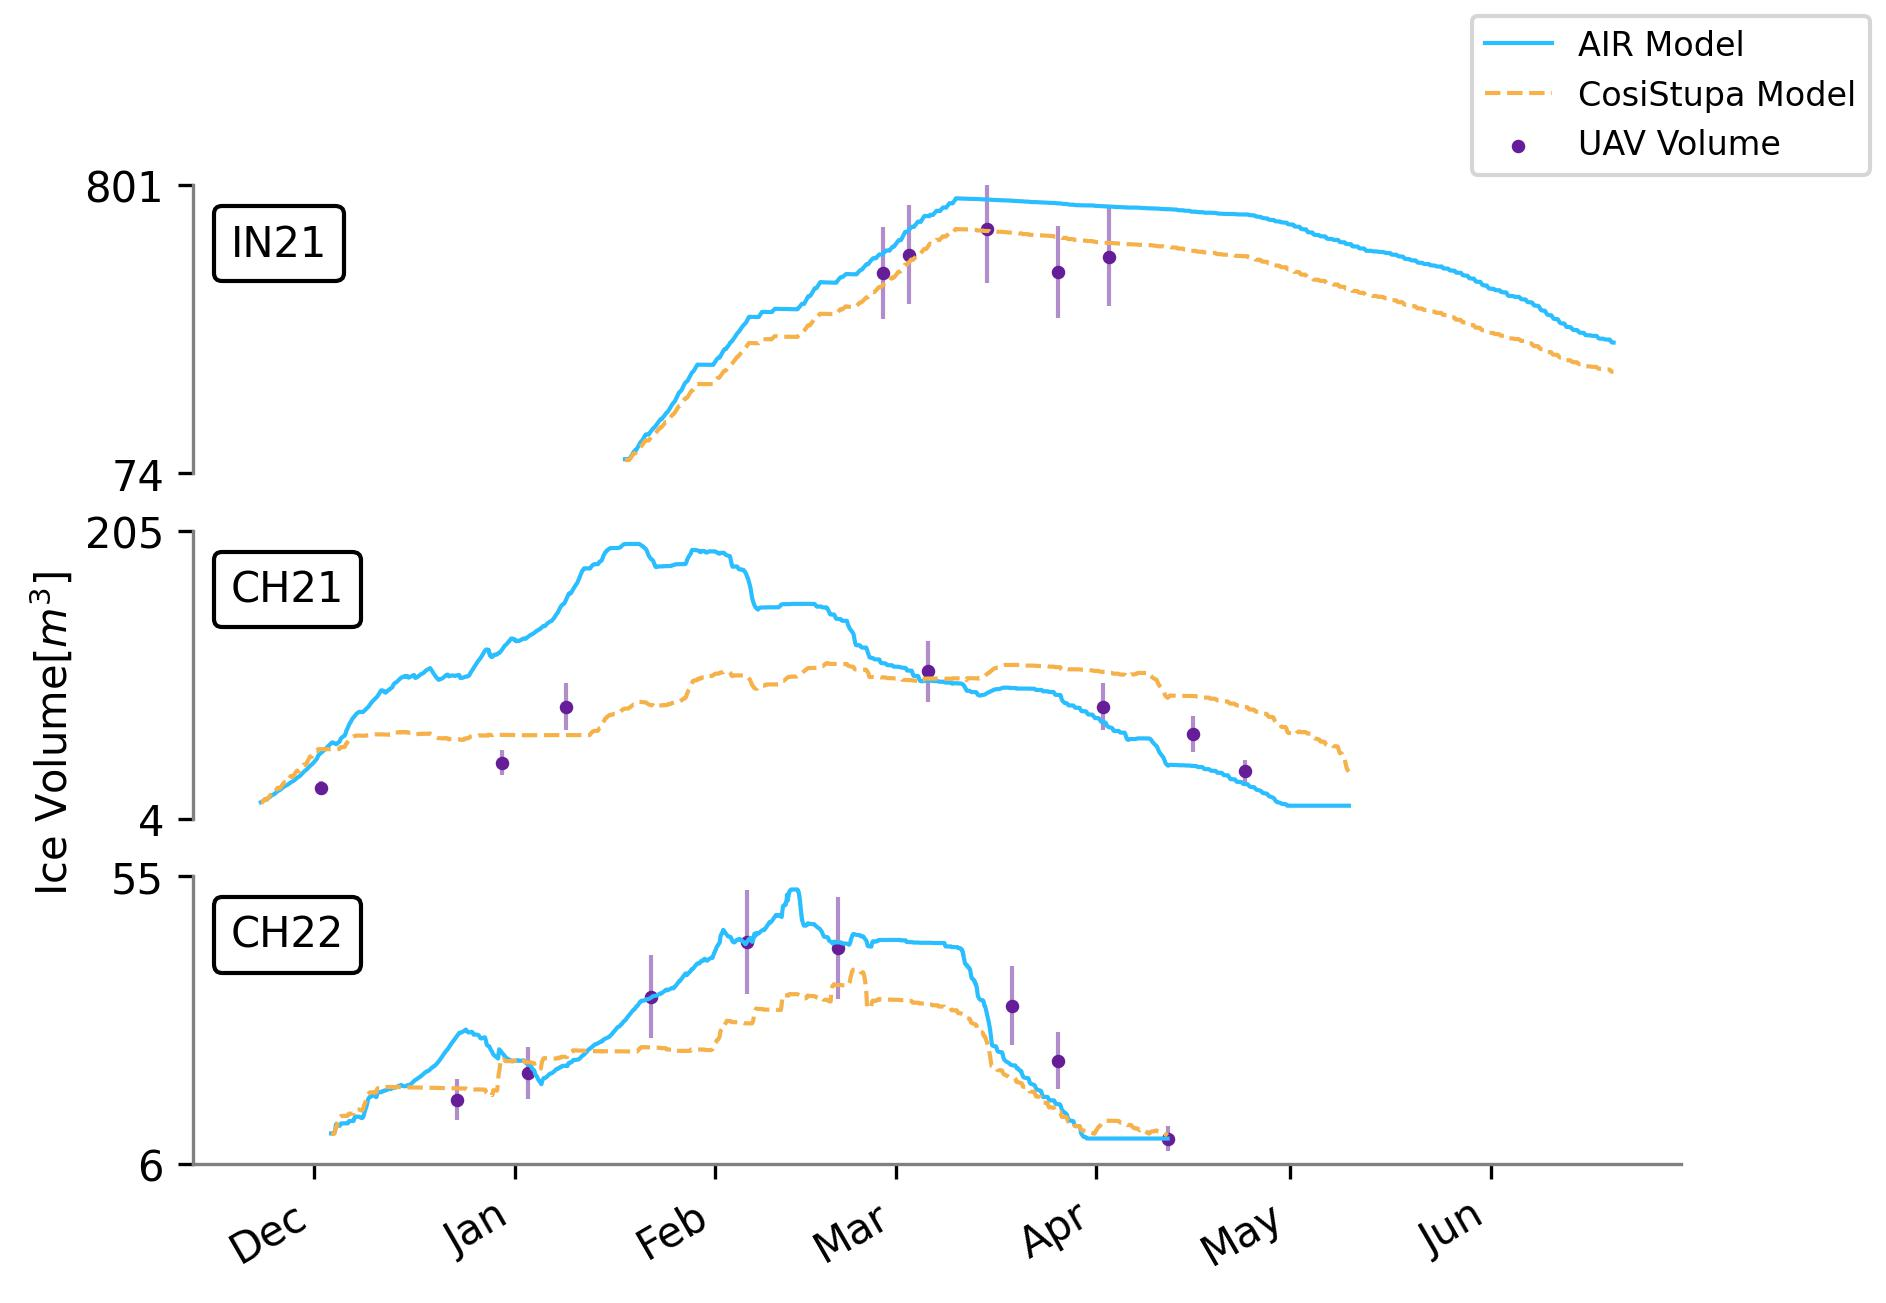
\includegraphics[width=\textwidth]{figs/model_compare.jpg}

	\caption{Comparison of volume estimates generated from the AIR and COSISTUPA models.}

	\label{fig:Cosistupa}
\end{figure}

We consider the COSISTUPA model to be the better one among the three models due to these three reasons:

\begin{itemize}

	\item \textbf{Better spatial temperature and density resolution} : It provides temperature and density
	      information of subsurface layers of the AIR. In contrast, the AIR model only computes the bulk and the
	      surface temperature. Moreover, COSISTUPA is better able to approximate bulk density since it has records of
	      previous snowfall events in its subsurface layers.

	\item \textbf{Better parametrization of snowfall} : The densification and albedo decay of snowfall are better
	      handled in COSISTUPA due to its awareness of the snowfall content in each of its subsurface layers.

	\item \textbf{Better validation} : COSISTUPA, being a model derived from COSIPY is expected to validate better
	      since the core parametrizations are unchanged and have been extensively validated within other studies \citep{arndtAtmosphereDrivenMassBalance2021}.

	\item \textbf{Future support} : COSISTUPA will be extensively supported in the future through the COSIPY
	      community.

\end{itemize}


